% Author: PokMan Ho pok.ho19@imperial.ac.uk
% Script: normality.tex
% Desc: normality test section
% Input: none
% Output: none
% Arguments: 0
% Date: Jan 2020

\documentclass[../note.tex]{subfiles} %% use packages & commands as this main file

\begin{document}

\section{Data Normality}
If you want to use parametric tests on your numeric data, this part is super-important and should be the first test to be carried out before going onto the statistical test itself.  There are three ways to test for data normality and your data have to pass at least two (just a convention, the majority rules) to gain a ``normal-distributed" data status.

\subsection{Shapiro test}
This is the most convenient and objective way to test for numeric variable normality.  However in R there is a limitation: the number of data can only be between 3 and 5000.  This maybe one of the few occasions you'd like to see non-significant p-value.

The code (in ``stats" package\autocite{Rcore}) is
\begin{code}
shapiro.test(a\$dep)\\
\# testing hypothesis (p $<$ 0.05): the data is skewed\\
\# Hence null hypothesis (p-val $>$ 0.05): the data is not skewed (i.e. normally-distributed).
\end{code}

\subsection{qq-plot}
\begin{code}
library(car)\\
qqPlot(a\$dep)\\
\# indicated mean with 95\% interval
\end{code}
There is also a base R version of qq-plot.  However the base R version requires more lines of code and lack a 95\% confidence interval for judging normality, hence it is not effective and efficient to spend time on coding it.  Below is a sample of the qqPlot from ``car" package on normality of the dependent variable of our sample dependent variable data:
\begin{center}
    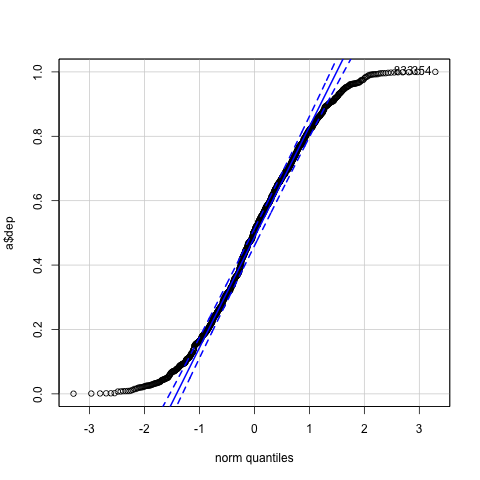
\includegraphics[width=.5\linewidth]{../graph/qqPlot.png}
\end{center}

In the above graph, the solid line is the mean and dashed lines indicate the 95\% confidence interval of that mean based on the input data.  Data is called ``normally-distributed" only when all plotted points are within the 95\% confidence interval.  Hence our dependent variable in the sample data is not normally-distributed judged by the qqPlot.

\subsection{Histogram}
This is the easiest method. However it requires you to interpret and judge the normality of data (subjectivity \& biases??).  So generally it is not recommended by the author unless one or more methods listed above cannot function as it should be, or they disagree with each other.  As we all should have known, histogram are plotting frequencies on continuous numeric values.  Thus the variable must be numeric data type [use as.numeric(variable) command if needed]

The code (in ``graphics" package\autocite{Rcore}) is
\begin{code}
hist(a\$dep)
\end{code}
\begin{center}
    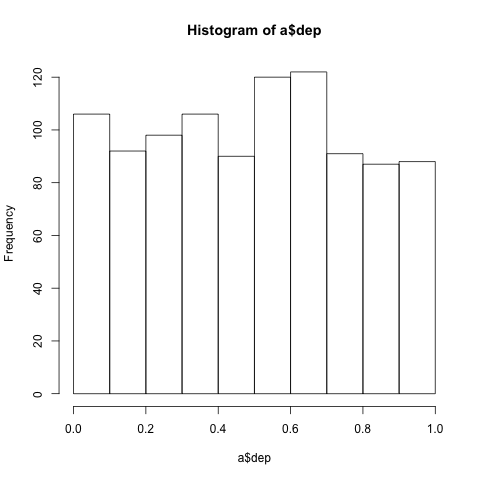
\includegraphics[width=.5\linewidth]{../graph/histogram.png}
\end{center}

In the above graph, if it does not look like normally-distributed, the data is considered as ``not normally-distributed".

\end{document}